%  -----------------------------------------------------------------------------
%  Author         : Bimalka Piyaruwan Thalagala
%  GitHub         : https://github.com/bimalka98
%  Date Created   : 11/8/2021
%  Last Modified  :
%  -----------------------------------------------------------------------------

\documentclass[a4paper,11pt]{article}%,twocolumn
%% packages

\usepackage{blindtext} % needed for creating dummy text passages
%\usepackage{ngerman} % needed for German default language
\usepackage{amsmath} % needed for command eqref
\usepackage{amssymb} % needed for math fonts
\usepackage[colorlinks=true,breaklinks]{hyperref} % needed for creating hyperlinks in the document, the option colorlinks=true gets rid of the awful boxes, breaklinks breaks lonkg links (list of figures), and ngerman sets everything for german as default hyperlinks language
\usepackage[hyphenbreaks]{breakurl} % ben�tigt f�r das Brechen von URLs in Literaturreferenzen, hyphenbreaks auch bei links, die �ber eine Seite gehen (mit hyphenation).
\usepackage{xcolor}
\definecolor{c1}{rgb}{0,0,1} % blue
\definecolor{c2}{rgb}{0,0.3,0.9} % light blue
\definecolor{c3}{rgb}{0.3,0,0.9} % red blue
\hypersetup{
    linkcolor={c1}, % internal links
    citecolor={c2}, % citations
    urlcolor={c3} % external links/urls
}
%\usepackage{cite} % needed for cite
\usepackage[square,authoryear]{natbib} % needed for cite and abbrvnat bibliography style
\usepackage[nottoc]{tocbibind} % needed for displaying bibliography and other in the table of contents
\usepackage{graphicx} % needed for \includegraphics 
\usepackage{longtable} % needed for long tables over pages
\usepackage{bigstrut} % needed for the command \bigstrut
\usepackage{enumerate} % needed for some options in enumerate
%\usepackage{todonotes} % needed for todos
\usepackage{makeidx} % needed for creating an index
\makeindex
\usepackage{gensymb}
\usepackage{url}
\usepackage{psfrag}
\usepackage{multirow}
\usepackage{subfigure}
%% page settings

\usepackage[top=15mm, bottom=15mm,left=20mm,right=20mm]{geometry} % needed for page border settings
\parindent=0mm % for space of first line of new text block
\sloppy % for writing with hyphenless justification (tries to)
\hyphenation{} % use hyphenation of tolerance parametershttp://www.jr-x.de/publikationen/latex/tipps/zeilenumbruch.html
\hyphenpenalty=10000
\exhyphenpenalty=10000
\usepackage{fancyhdr} % needed for head and foot options
%% my macros

%% Text fomats
\newcommand{\tbi}[1]{\textbf{\textit{#1}}}

%% Math fonts
\newcommand{\bbA}{\mathbb{A}}
\newcommand{\bbB}{\mathbb{B}}
\newcommand{\bbC}{\mathbb{C}}
\newcommand{\bbD}{\mathbb{D}}
\newcommand{\bbE}{\mathbb{E}}
\newcommand{\bbF}{\mathbb{F}}
\newcommand{\bbG}{\mathbb{G}}
\newcommand{\bbH}{\mathbb{H}}
\newcommand{\bbI}{\mathbb{I}}
\newcommand{\bbJ}{\mathbb{J}}
\newcommand{\bbK}{\mathbb{K}}
\newcommand{\bbL}{\mathbb{L}}
\newcommand{\bbM}{\mathbb{M}}
\newcommand{\bbN}{\mathbb{N}}
\newcommand{\bbO}{\mathbb{O}}
\newcommand{\bbP}{\mathbb{P}}
\newcommand{\bbQ}{\mathbb{Q}}
\newcommand{\bbR}{\mathbb{R}}
\newcommand{\bbS}{\mathbb{S}}
\newcommand{\bbT}{\mathbb{T}}
\newcommand{\bbU}{\mathbb{U}}
\newcommand{\bbV}{\mathbb{V}}
\newcommand{\bbW}{\mathbb{W}}
\newcommand{\bbX}{\mathbb{X}}
\newcommand{\bbY}{\mathbb{Y}}
\newcommand{\bbZ}{\mathbb{Z}}
\usepackage[ framed, numbered]{matlab-prettifier}%framed,%
\usepackage{listings}
\usepackage{pythonhighlight}
\usepackage{pdfpages}

\begin{document}

\begin{titlepage}
\center % Center everything on the page

%-------------------------------------------------------------------------------------
%	HEADING SECTIONS
%------------------------------------------------------------------------------------
\textbf{\large Department of Electronic and Telecommunication Engineering}\\[0.5cm]
\textbf{\Large University of Moratuwa, Sri Lanka}\\[1cm]
\textbf{\large EN 2053 - Communication Systems and Networks}\\[2cm]

\includegraphics[width=0.3\textwidth]{figures/uomlogo}\\[2cm]

	
%-------------------------------------------------------------------------------------
%	TITLE SECTION
%------------------------------------------------------------------------------------
\textbf{\Huge Modelling Propagation Losses and MANETs}\\[0.5cm]
\textbf{\Large Assignment 2}\\[5cm]


%----------------------------------------------------------------------------------------
%	MEMBERS SECTION
%----------------------------------------------------------------------------------------

\textbf{\large Submitted by}\\[0.5cm]
\begin{minipage}{0.2\textwidth}
	\begin{flushleft}
		{\large Thalagala B.P.}\\[4mm]
		{\large Sauranga H.W.C.}\\[4mm]
		
		
	\end{flushleft}
\end{minipage}
\hspace{5mm}
\begin{minipage}{0.2\textwidth}
	\begin{flushright}
		{\large 180631J }\\[4mm]
		{\large 180574K }\\[4mm]
		
	\end{flushright}
\end{minipage}\\[1.5cm]

%----------------------------------------------------------------------------------------
%	DATE SECTION
%----------------------------------------------------------------------------------------
\textbf{\large Submitted on}\\[0.5cm]
\textbf{\Large \today} % Date, change the \today to a set date if you want to be precise

%----------------------------------------------------------------------------------------

\vfill % Fill the rest of the page with whitespace

\end{titlepage}




\pagebreak
%%-----------------------------------------------------------------------
\includepdf[pages=-, width=\textwidth]{code/answers.pdf}



\section*{Question 4}
\subsection*{(a) The sequence of signals (waveforms) corresponding to the binary sequence}

Please note that when plotting the below figure following values were assumed for the parameters.\\

\begin{tabular}{l l}
	Bit interval ($T_b$) & 1 $s$ \\
	Symbol interval  (T) &$2 \times T_b = $  2 $s$
\end{tabular}

\begin{figure}[!h]
	\centering
	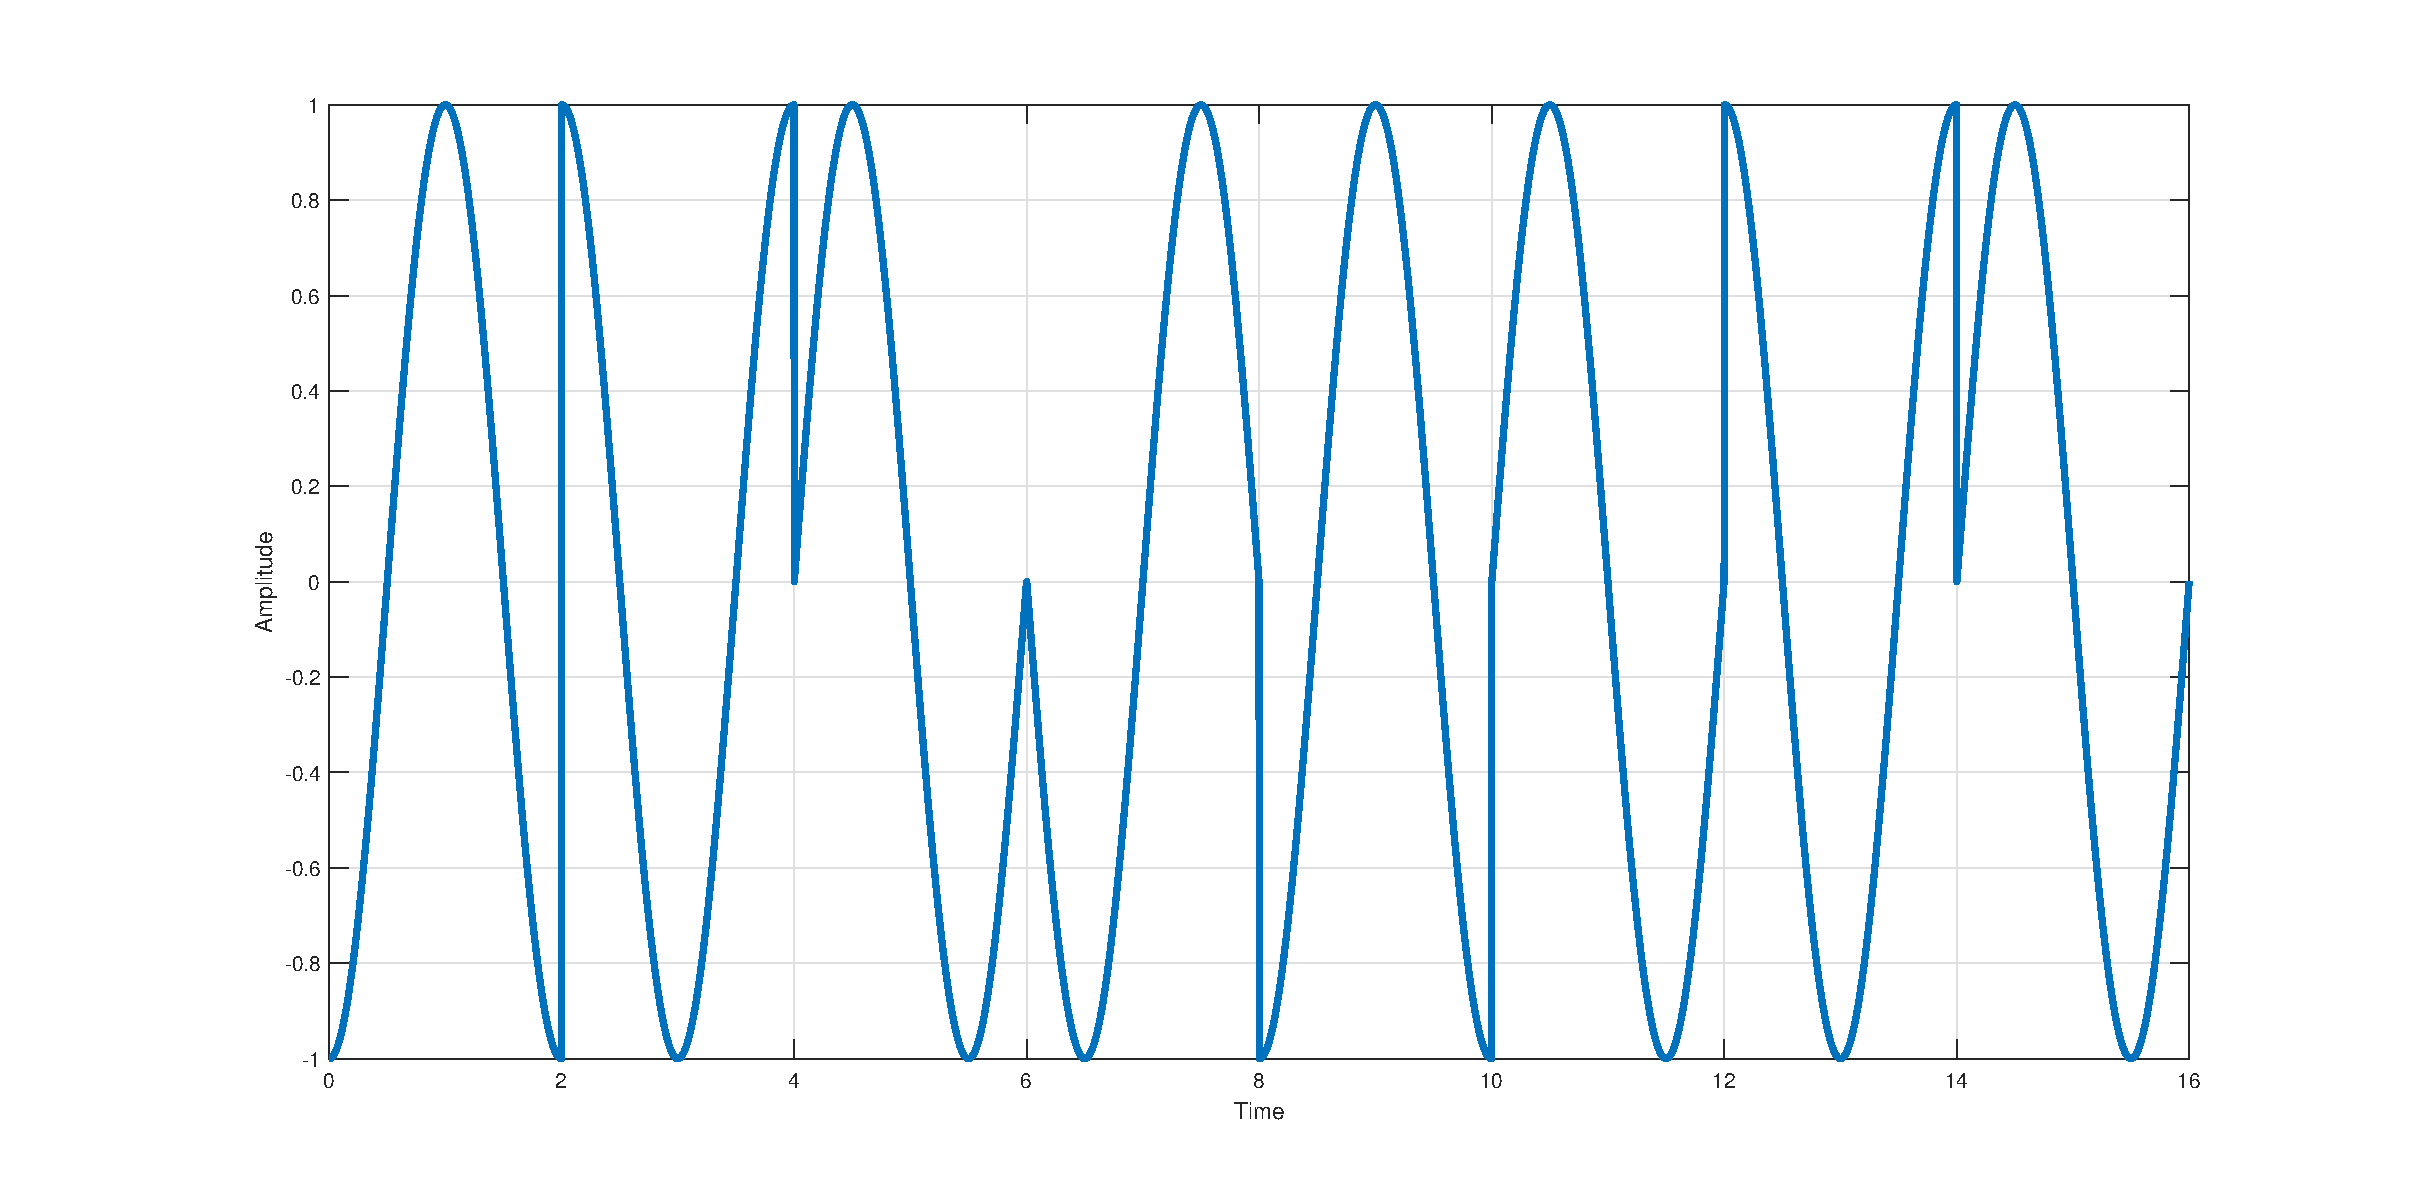
\includegraphics[scale=0.35]{figures/fig4a}
\end{figure}

\lstinputlisting[basicstyle = \mlttfamily\scriptsize , style = Matlab-editor]{code/codea.m}

\pagebreak
\subsection*{(b) The Quaternary MSK phase trajectory}
Please note that when plotting the below figure following values were assumed for the parameters.\\

\begin{tabular}{l l}
	Bit interval ($T_b$) & 1 $s$ \\
	Symbol interval  (T) &$2 \times T_b = $  2 $s$
\end{tabular}

\begin{figure}[!h]
	\centering
	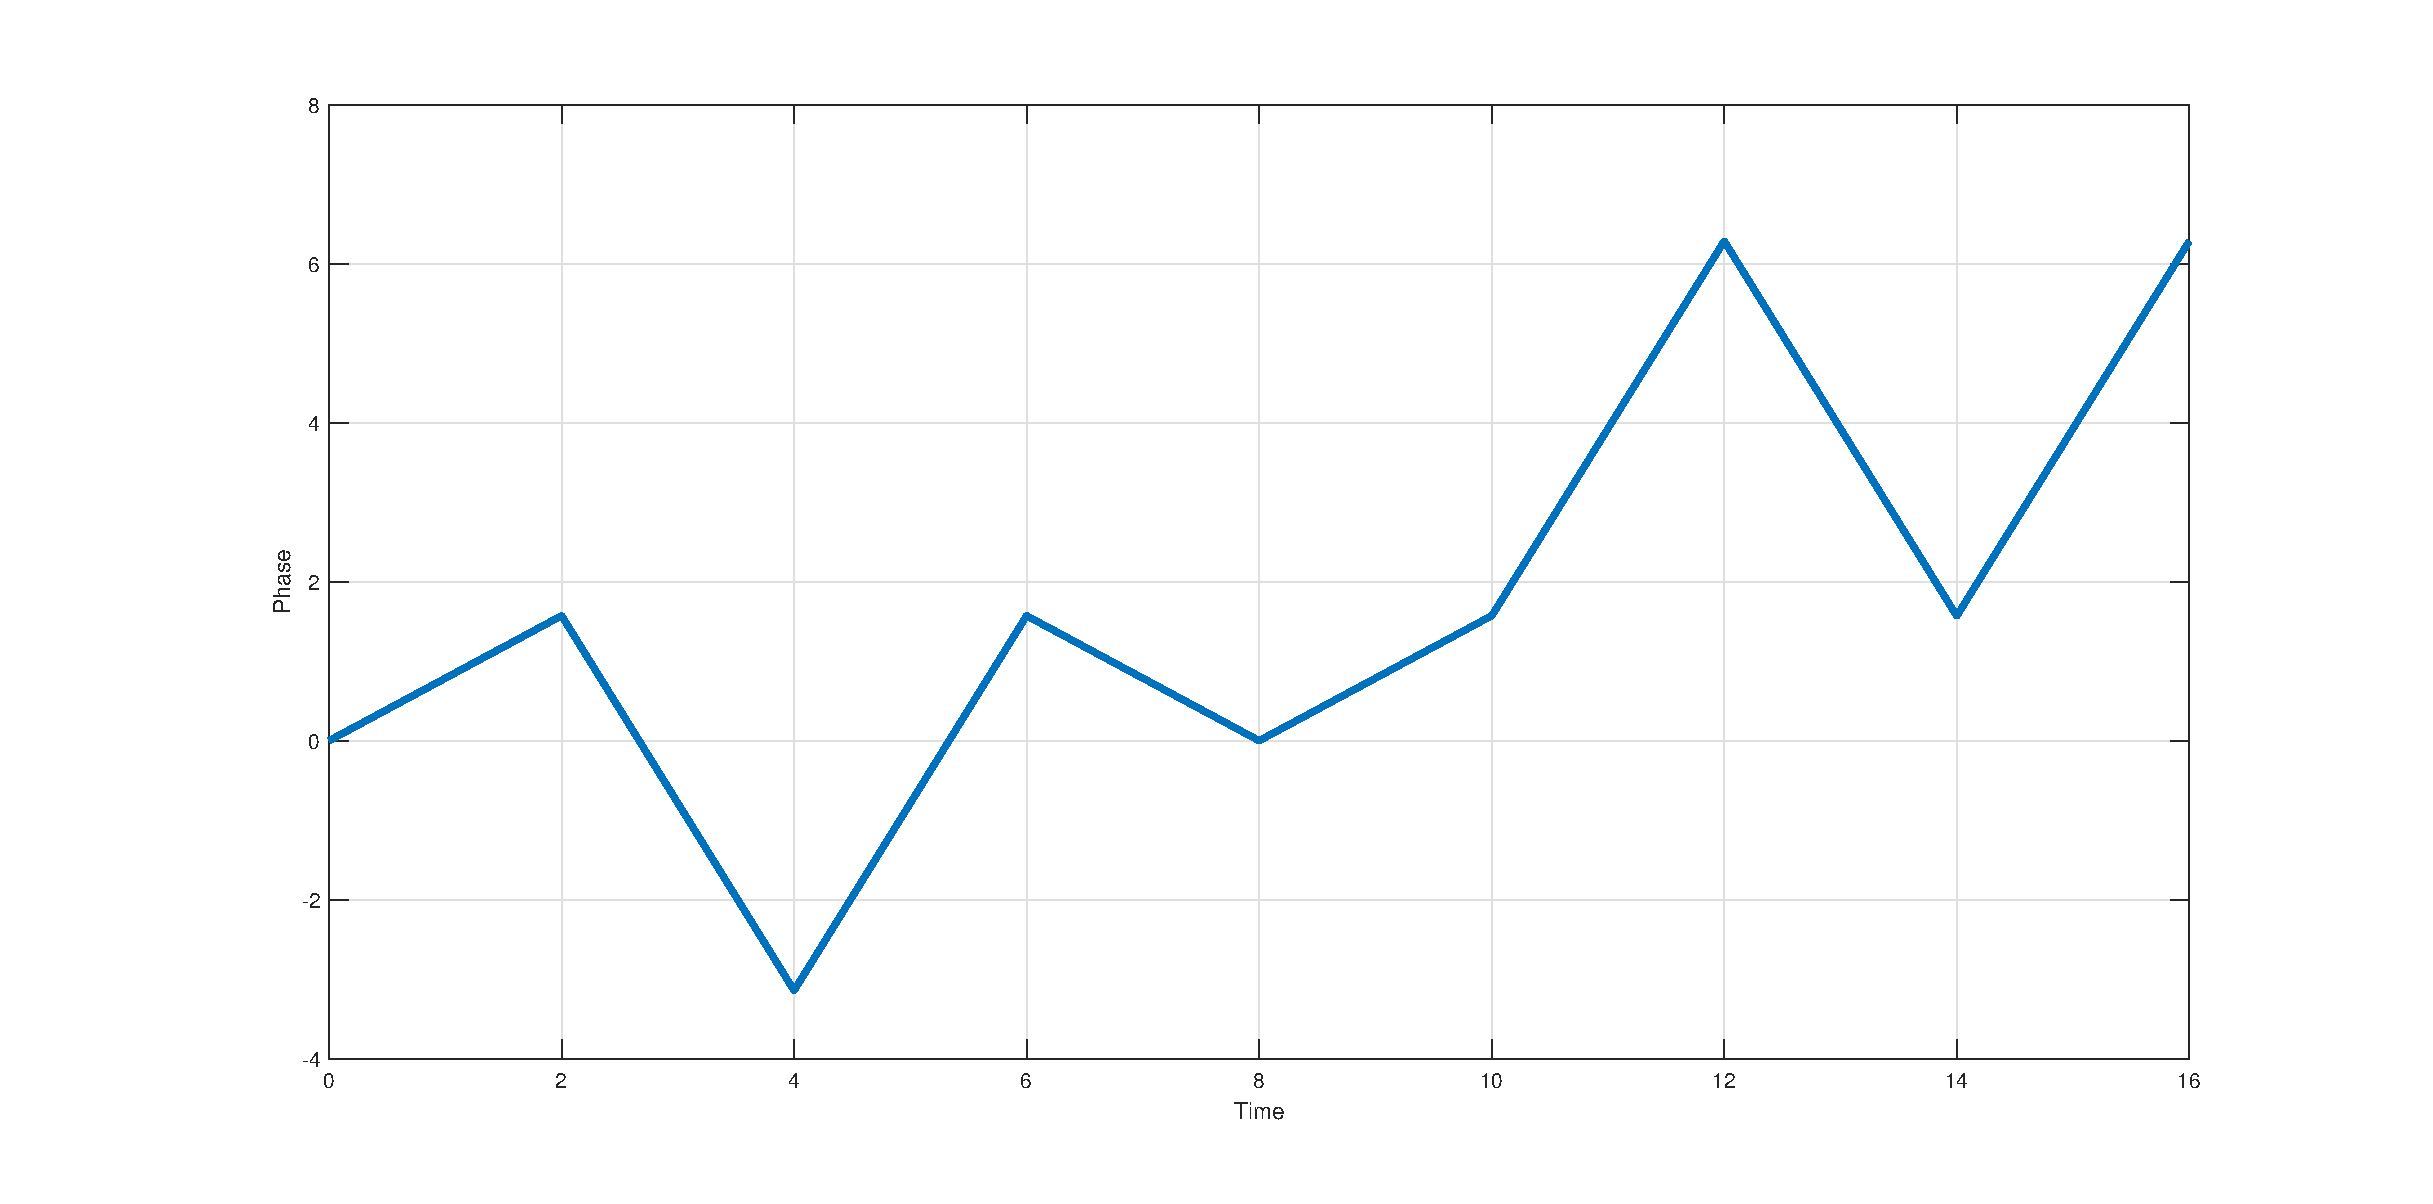
\includegraphics[scale=0.35]{figures/fig4b}
\end{figure}

\lstinputlisting[basicstyle = \mlttfamily\scriptsize , style = Matlab-editor]{code/codeb.m}

\pagebreak
\subsection*{(c) The Quaternary MSK waveform corresponding to the binary sequence}
Please note that when plotting the below figure following values were assumed for the parameters.\\

\begin{tabular}{l l}
	Bit interval ($T_b$) & 1 $s$ \\
	Symbol interval  (T) &$2 \times T_b = $  2 $s$
\end{tabular}

\begin{figure}[!h]
	\centering
	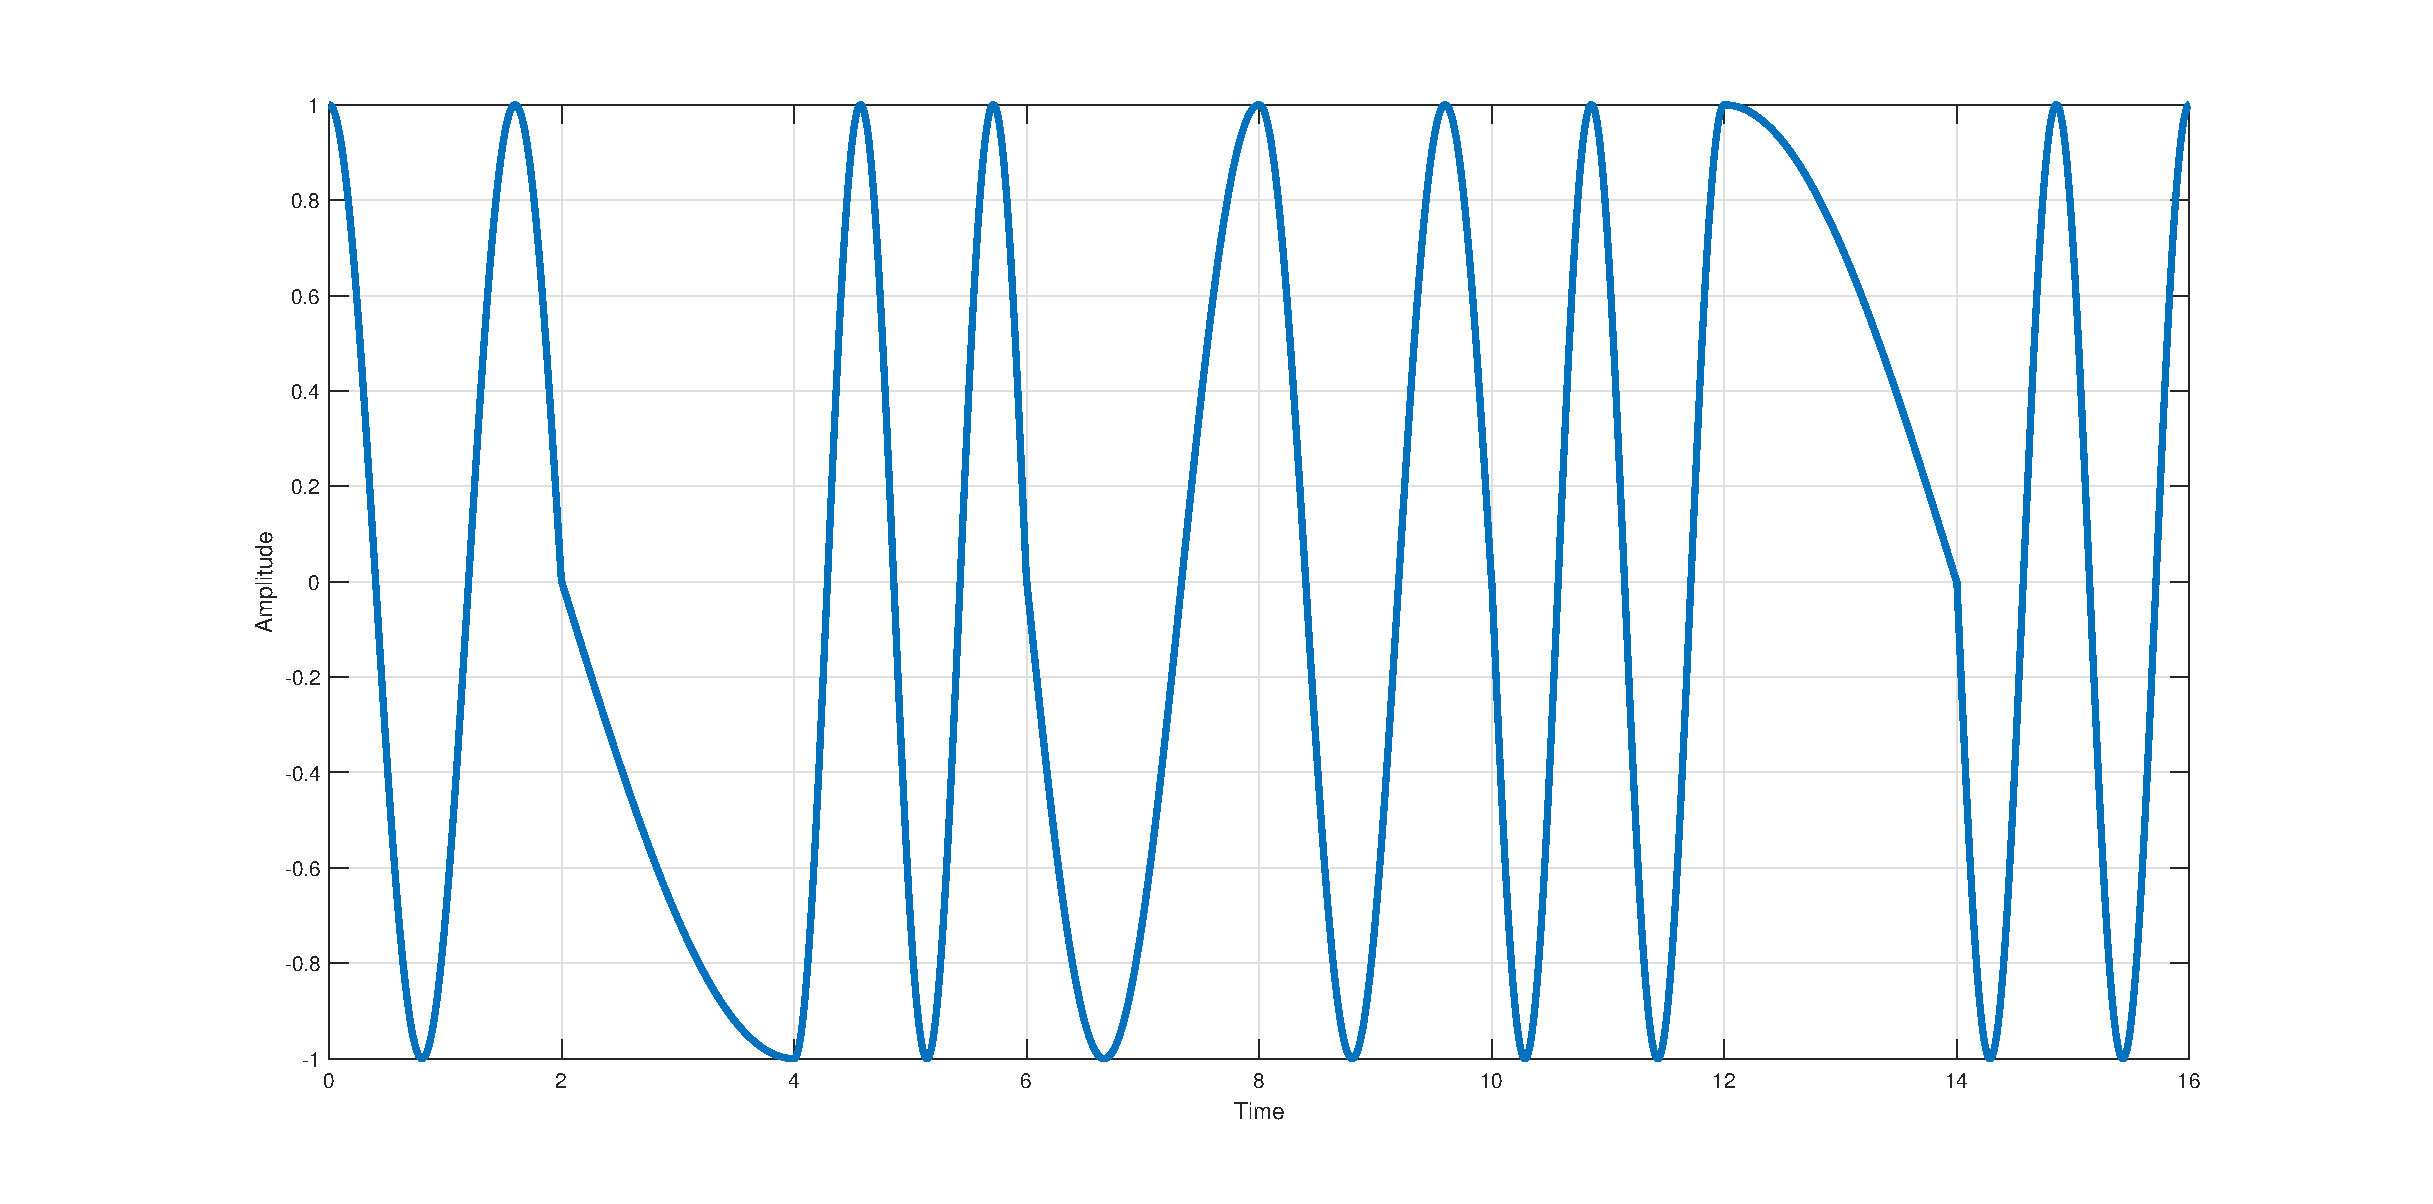
\includegraphics[scale=0.35]{figures/fig4c}
\end{figure}

\lstinputlisting[basicstyle = \mlttfamily\scriptsize , style = Matlab-editor]{code/codec.m}
%---------------------------------------------------------------------------
\end{document}
